\twocolumn
\section{Introduction}
\epigraph{\small \justify``Two things fill the mind with ever new and increasing admiration and awe, the more often and steadily we reflect upon them: the starry heavens above me and the moral law within me.''}{Immanuel Kant (1724-1804)\\\textit{Critique of Practical Reason, 1788}}

\subsection{Background}
The notion of colour sends a philosopher pondering about its ontology and the relation with the mind, while the impressionists akin to Monet, are busy evoking awe in the play with the pigments. And there are the astronomers who have precisely defined colours in terms of the electromagnetic spectrum\footnote{The dispersion prism breaking light into its respective colours are famously illustrated in pop-culture. For instance, in an album cover of the English rock band Pink-Floyd. This phenomenon was demonstrated and explicated by Newton 300 years ago.} of light. Alex Filippenko, the professor of astronomy at UC Berkeley put it aptly; light is the supreme informant, a goldmine for astronomers. Its colours are the embedded knowledge of the celestial bodies \parencite[96]{filippenko_great_2007}.

Astronomers have been training their telescopes to collect light from galactic objects and the quality and quantity of data have improved with the improvement of their telescopes from Galileo's refractive lens to the modern adaptive optics and onward to the more advanced charged-couple detectors. The last decade has seen a proliferation of computing power, combined with modern astronomy's advanced high-throughput telescopes, the summation of data generated is humongous \parencite[43]{ivezic_statistics_2014}. Thence emerges an inevitable problem in analysing these vast heaps of data and then mining out the embedded knowledge to facilitate further predictions.

In this study, I use the publicly released dataset on distant galaxies, administered by and collected from the \emph{Sloan Digital Sky Survey} \parencite{stoughton_sloan_2002} including the public citizen science project, \emph{Galaxy Zoo} \parencite{lintott_galaxy_2008, raddick_galaxy_2010, lintott_galaxy_2011, raddick_galaxy_2013}. I look particularly at the flux magnitudes of galaxies and take in as features the magnitudes across 5 colours or bands in the electromagnetic spectrum. Using the co-relation between flux magnitudes and redshifts, similarly flux magnitudes with the morphology of the galaxy, I employ machine learning models to predict the target features, namely redshifts and morphology.

\subsection{Aim \& Objectives}
The primary aim of my dissertation is to discover whether ensemble classifiers improve the prediction accuracy of galaxy redshifts and morphology, based on their apparent flux magnitudes. And if so, by what factor?

In the process, I strive to garner skills in applied machine learning and also insights in astronomy. Other learnings include the method of conducting empirical research while developing technical soundness and an incisive mind for problem-solving. Moreover, I regard this dissertation as an encouragement for students to engage in multi-disciplinary approach to problem resolution.

\subsubsection{Technical Objectives.}
\begin{enumerate}
\item Conduct Literature Review
	\begin{enumerate}
		\item Review  astronomy research on galaxy spectroscopy.
		\item Review Machine Learning applications in astronomy.
	\end{enumerate}
\item Perform Regression to Predict Redshifts
\begin{enumerate}
	\item Prepare SDSS dataset.
	\item Perform Hold-out Validation.
	\item Model's performance.
	\item Overfitting assessment.
	\item Optimum Tree-depth.
	\item Perform K-Fold Cross Validation.
\end{enumerate}
\item Perform Classification to predict Galaxy Morphology.
\begin{enumerate}
	\item Prepare Galaxy Zoo dataset.
	\item Engineer \& Extract Features.
	\item Perform hold-out validation.
	\item Assess decision tree's performance.
	\item Perform Hold-out Validation.
	\item Perform Ensemble learning with Random Forest.
	\item Assess Random Forest's Performance.
	\item Perform Compare Performance of DT \& RF.
\end{enumerate}
\end{enumerate}

\subsubsection{Personal Objectives}
\begin{enumerate}
	\item Understand the nature of learning.
	\item Be able to identify ML solvable problems
	\item Garner Applied ML Skills
	\item Foster an incisive mind
	\item Garner applied ML skills
	\item Build a scholarly Portfolio
	\item Assimilate cosmological studies
\end{enumerate}

\subsubsection{Academic Objectives}
\begin{enumerate}
	\item Grok Research Methodology
	\item Grok Data-driven Astronomy
	\item Learn \& Apply scientific computing with Python.
	\item Cognize machine learning techniques.
	\item Synthesize Knowledge.
	\item Fulfill the Requirement for the Honors degree.
	\item Qualify as a Graduate.
\end{enumerate}
\subsection{Overview}
\begin{figure}[H]
	\centering
	\frame{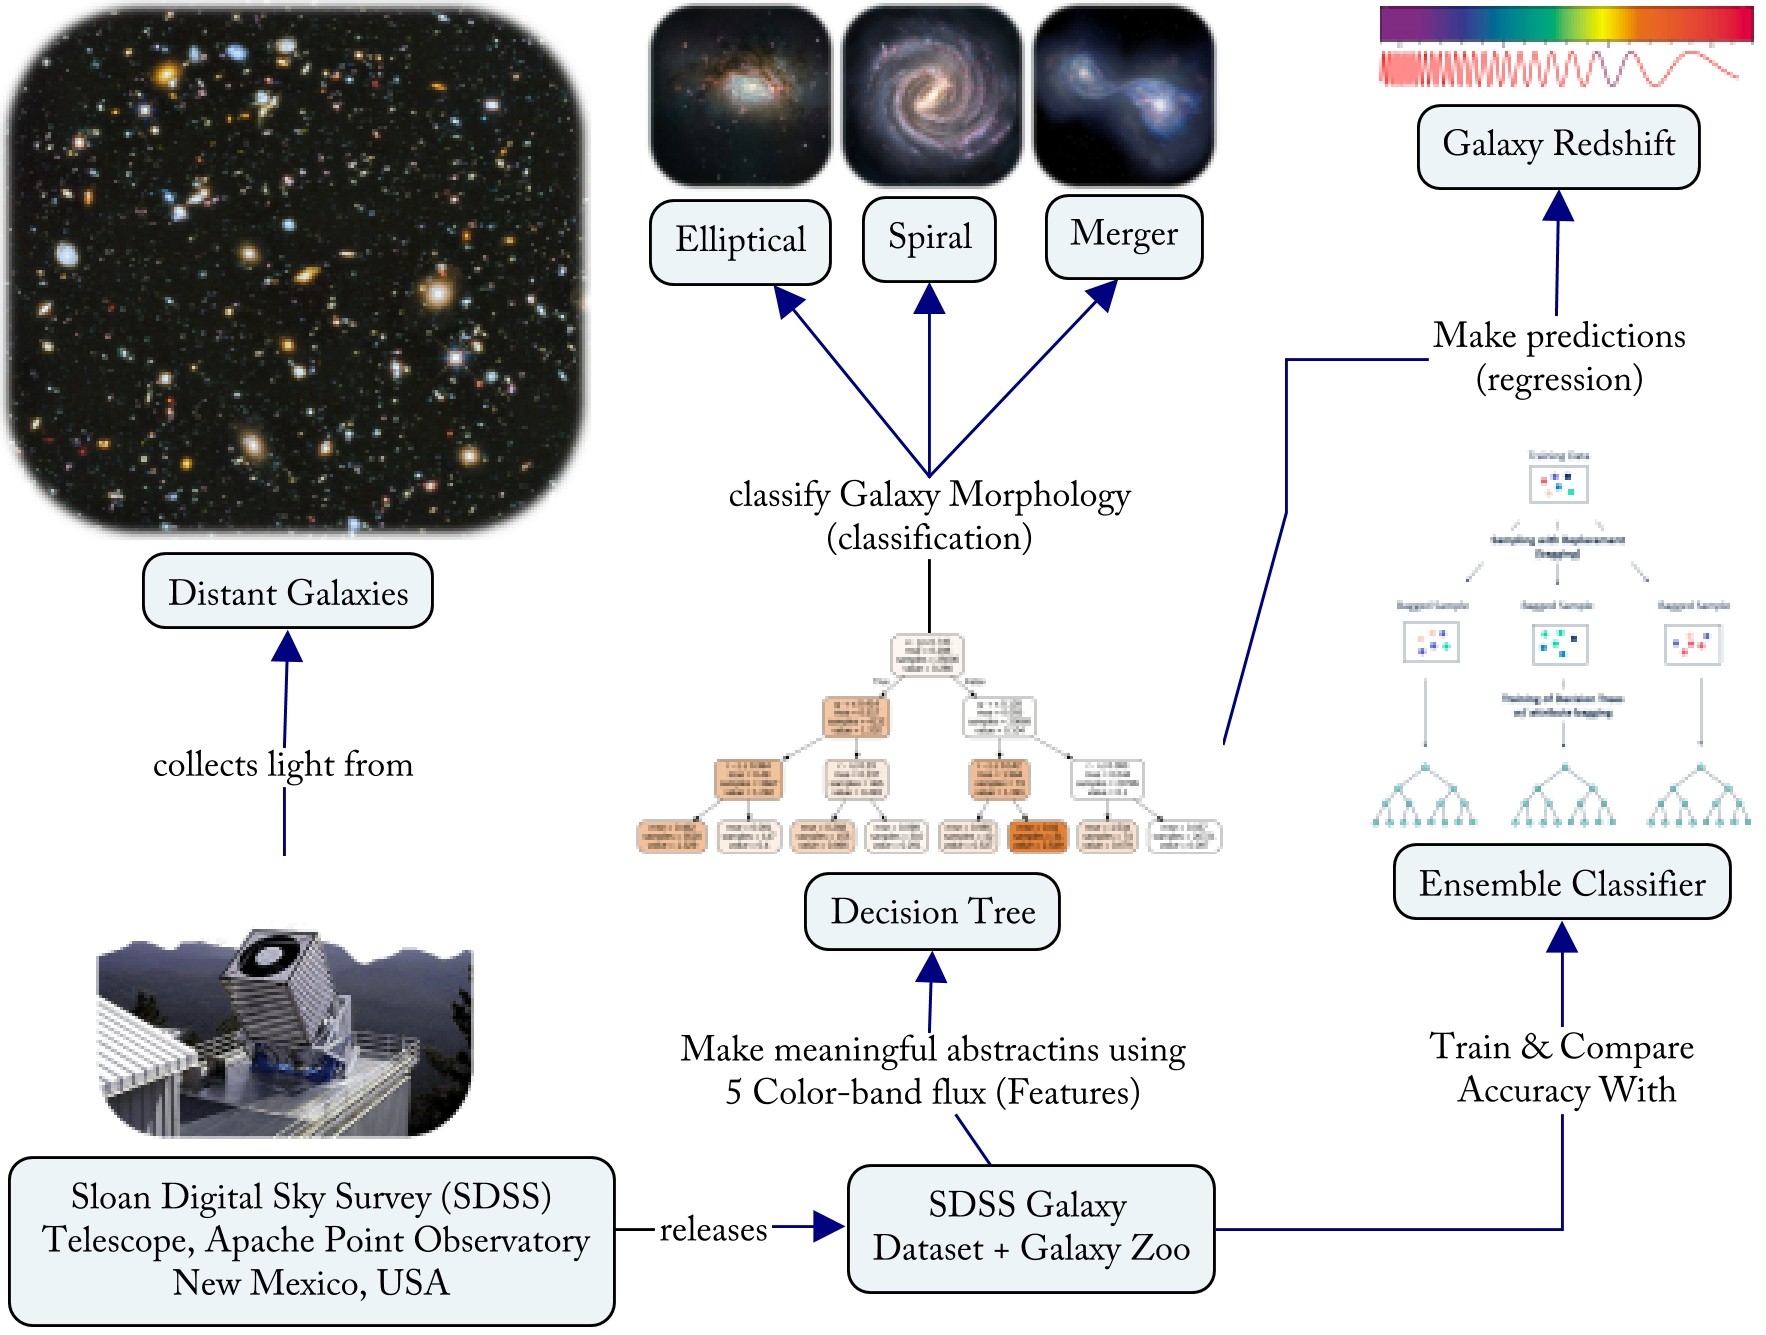
\includegraphics[width=\linewidth, height=\textheight, keepaspectratio]{images/rp.jpg}}
	\caption{Rich Picture depicting the overview of the dissertation project. Image Credit/Reference: Distant Galaxies \parencite{nasa_hubblesite:_2004}, Elliptical \parencite{nasa_hubble_2016}, Spiral \parencite{nasa/jpl_milky_2019}, Merger \parencite{evan_gough_artists_2019}, Sloan Telescope \parencite{ieee_computer_society_digital_liibrary_ieee_1999}}
\end{figure}
One of the frustrations of an observational science like astronomy is we can't set up experiments in the lab. We can't control the unknown parameters to test hypotheses or use physical equipment like rulers to measure distances. Instead we have to cleverly construct observations to collect data that will allow us to answer our questions.

It is relatively straightforward for a person with the help of a computer to measure a redshift from a galaxy with an observed spectrum and hence work out how far away the galaxy is. But many galaxies have not been observed spectroscopically, we only have images. In addition, the sheer number of galaxies in these surveys makes this task impractical to do by hand.  In the first part of my research, I shall task machine learning to calculate the redshift of galaxies from their measured colours .

In this study, I shall employ decision trees to calculate the redshift of galaxies from the Sloan Digital Sky Survey. Let's use this example to work through what the process of supervised machine learning looks like. Getting the methodology right is critical and we'll discuss some of the pitfalls in later sections. I start with a sample of galaxies for which the answer is already known. Such a sample is called the gold standard. These are galaxies with measured spectroscopic redshifts. Typically quite a large sample is needed because the learner needs to be able to see enough instances of each type of object and its properties to correctly model and then predict the correct results. In addition to the regression of redshifts, I also task the decision tree to classify galaxies based on their morphologies. The same features of flux across the colour bands are used.

\subsection{Feature Extraction}
The next step is to extract features that represent the input data in some way. Sometimes it is obvious how to do this because the manual classification scheme we use is designed by specific features. In this study, colours measured by comparing the magnitudes from five different Sloan filters. U, G, R, I and Z are used. Each filter measures the light from the galaxy in a particular wavelength range. To calculate colours, astronomers subtract the magnitudes measured in neighbouring filters. For example, U minus G or I minus Z.

\subsection{Algorithm Selection}
Decision tree is selected as the regresison classifier. Other algorithms like neural networks, random forests and naive Bayes classifiers can also be used. For some tasks, Naive Bayes classifiers are typically very fast but don't have great accuracy. Whereas random forests classify have high accuracy but can be much slower to run. One of the reasons decision trees are great is that the model they produce is quite intuitive for humans to understand. In fact, the decision tree was involved in the kinds of schemes scientists have been using for generations. For example, in developing taxonomies in biology.

\subsection{Training \& Accuracy}
The process of training basically consists of building a model between the inputs and the result. The nature of the model depends on the classification algorithm being used, the big question when at the onset of training a classifier is, how accurate is it? It is worth thinking about how it applies in light of humans. In the early days of classification, most objects would only have been classified once. Classifiers like Annie Cannon were extremely expert and very careful. So their classifications were probably pretty reliable. But there's no doubt that even the most diligent human classifiers can make mistakes. An obvious way of evaluating the reliability of a human classifier would be to get another expert to classify the same set of data and compare their results. This would give  a measure of how reliable their classifications are. If a classifier makes a mistake, an object of category A could be accidentally classified as category B. When all objects must be classified, each mistake introduces two classification errors, an extra B, a false positive and a missing A, a false negative. Machine learning researchers typically quantify the reliability of a classifier using two measures, precision and recall, and we'll explore these in the activities.

\subsection{Cross-Validatioin}
So how do we know our classifier will be accurate on unknown data if it's just trained on one data set? To answer this, I have used n-fold cross-validation. You split your sample of galaxies with known redshifts into ten sets or folds, which are usually chosen randomly. You then train your classifier on the galaxies in nine of these sets and test it on the galaxies in the tenth set and record the precision and recall. You repeat this process for each fold and calculate the mean and the standard deviation, which is how you get the name 10-fold Cross-Validation. You've now developed a system that learns the classificational regression from data and can evaluate how reliable it is. You can now run it on some unknown galaxies, determine their redshifts and estimate to make their errors.